%%
%% Copyright 2019 Elsevier Ltd
%%
%%
%%%%%%%%%%%%%%%%%%%%%%%%%%%% ! ! ! SUBMISSION CHECKLIST ! ! ! %%%%%%%%%%%%%%%%%%%%%%%%%%%%
%%
%% Please confirm that your submission follows all the requirements of the guidelines,
%% including the submission checklist:
%% _ Cover letter
%% _ Highlights
%% _ Authorship statement
%% _ The manuscript must be single column and double spaced
%% _ Reference must be in the author-date format
%% _ Code availability section
%%
%% *All the manuscripts in disagreement with the guidelines will be desk-rejected
%%  without editorial check.
%%
%% --------------------------------------
%%
%% This file is part of the 'CAS Bundle'.
%%
%% It may be distributed under the conditions of the LaTeX Project Public
%% License, either version 1.2 of this license or (at your option) any
%% later version.  The latest version of this license is in
%%    http://www.latex-project.org/lppl.txt
%% and version 1.2 or later is part of all distributions of LaTeX
%% version 1999/12/01 or later.
%%
%% The list of all files belonging to the 'CAS Bundle' is given in the
%% file `manifest.txt'.
%%
%% Template article for cas-sc documentclass for single column output.

%\documentclass[a4paper,fleqn,longmktitle]{cas-dc}
\documentclass[a4paper,fleqn]{cas-sc}

%% ── Font: Latin Modern (Type1 T1 fonts, avoids EC bitmap font issues)
\usepackage{lmodern}

%% ── Core packages ────────────────────────────────────────────────────────────
\usepackage[authoryear]{natbib}
\usepackage{graphicx}
\graphicspath{{../../}}
\usepackage{float}
\usepackage{algorithm}
\usepackage{algpseudocode}
\usepackage{color}
\usepackage{setspace}
%\usepackage[nomarkers,figuresonly]{endfloat}

%% ── Math ─────────────────────────────────────────────────────────────────────
\usepackage{amsmath}
\usepackage{amssymb}

%% ── Tables ───────────────────────────────────────────────────────────────────
\usepackage{booktabs}

%% ── Figures: subfigures ──────────────────────────────────────────────────────
\usepackage{subcaption}

%% ── TikZ diagrams ────────────────────────────────────────────────────────────
\usepackage{tikz}
\usetikzlibrary{arrows.meta, positioning, shapes.geometric, patterns, calc}

%% ── Cross-references ─────────────────────────────────────────────────────────
\usepackage[capitalize, noabbrev]{cleveref}

%% ── Miscellaneous ────────────────────────────────────────────────────────────
\usepackage{xspace}
\usepackage{lineno}
\renewcommand{\linenumberfont}{\normalfont\footnotesize\sffamily}
\linenumbers

%% ── Custom macros ────────────────────────────────────────────────────────────
\newcommand{\colorComments}{black}

%% Shorthand abbreviations with correct spacing
\newcommand{\eg}{e.g.\@\xspace}
\newcommand{\ie}{i.e.\@\xspace}

%% Architecture names
\newcommand{\EffNet}{EfficientNetB0\xspace}
\newcommand{\ResNet}{ResNet50\xspace}

%% Method / metric abbreviations
\newcommand{\PHNM}{Phase-1 HNM\xspace}
\newcommand{\PR}{PR-AUC\xspace}
\newcommand{\CP}{Clopper--Pearson\xspace}

%%%Author definitions (provided by CAS class)
\def\tsc#1{\csdef{#1}{\textsc{\lowercase{#1}}\xspace}}
\tsc{WGM}
\tsc{QE}
\tsc{EP}
\tsc{PMS}
\tsc{BEC}
\tsc{DE}
%%%

\begin{document}
\let\WriteBookmarks\relax
\def\floatpagepagefraction{1}
\def\textpagefraction{.001}
\shorttitle{Short title}
\shortauthors{short author name}

\title [mode = title]{Manuscript title - \LaTeX  template for Computers \& Geosciences  }


\author[1]{Author 1}[type=editor,
                        auid=000,bioid=1,orcid=0000-0000-0000-0000]
\credit{ Author 1 contribution  }

\author[2]{Author 2} 
\credit{Author 2 contribution }

\author[3]{Author 3}
\credit{Author 3 contribution}

\address[1]{Author 1 affiliation}
\address[2]{Author 2 affiliation}
\address[3]{Author 3 affiliation} 

\begin{abstract}
We introduce Phase-1 Hard Negative Mining (\PHNM{}), a confounder-targeted
resampling pipeline for street-level flood detection that exploits a partially
trained intermediate checkpoint to recover visual confounder candidates that a
fully converged model cannot provide.
Existing flood screening systems report aggregate accuracy or ROC-AUC, which
conceal category-level false positive rates and overstate discrimination on
class-imbalanced datasets.
We fine-tune \EffNet{} and \ResNet{} with a two-phase progressive transfer
learning protocol on 4,099 deduplicated street-level images spanning eight
non-flood categories including four water confounders, mine difficulty-ranked
candidates from the Phase-1 checkpoint, apply $5\times$ augmentation, and
retrain, ablating against extended-training and random-injection controls,
evaluating with \PR{} as primary metric and per-category false positive rates
with \CP{} 95\,\% binomial confidence intervals.
Both \EffNet{} (\PR{}$= 0.9976$, 97.8\,\% flood recall, 7\,FN) and \ResNet{}
(\PR{}$= 0.9991$, 97.2\,\% flood recall, 9\,FN) achieve strong baselines with
complementary tradeoffs: \EffNet{} captures more floods per threshold at
$\tau{=}0.5$ while \ResNet{} maintains a lower river false positive rate
(3.9\,\% vs.\ 9.2\,\%).
\PHNM{} resolves this tradeoff for \EffNet{}: difficulty-ranked selection
simultaneously improves flood recall to 99.1\,\% (3\,FN, 1 in 107) and reduces
river false positive rate from 9.2\,\% to 5.3\,\%, outperforming both extended
training and random injection ablation controls.
\end{abstract}
 
\begin{coverletter}

Dear Editors-in-Chief,
\newline
 
please find the enclosed manuscript "..." which we are submitting for exclusive consideration for publication in Computers \& Geosciences. We confirm that the submission follows all the requirements and includes all the items of the submission checklist.  
\newline
 
The manuscript presents ... 
\newline

We provide the source codes in a public repository with details listed in the section "Code availability".
\newline

Thanks for your consideration. 
\newline

Sincerely,
\newline

Authors names

Corresponding author affiliation and e-mail
\newline

\textbf{Delete before submission:}

Please confirm that your submission follows all the requirements of the guidelines, including the submission checklist:

- Cover letter

- Highlights

- Authorship statement

- The manuscript must be single column and double spaced

- Reference must be in the author-date format

- Code availability section 

*The manuscripts that do meet the requirement guidelines will be desk-rejected.



\end{coverletter}

 
\begin{highlights}
\item Phase-1 Hard Negative Mining exploits an intermediate checkpoint to mine visual confounder candidates that a fully-converged model cannot provide.
\item River images are the dominant false-positive confounder; per-category FP rates with Clopper-Pearson CIs quantify this precisely.
\item P1-HNM simultaneously improves EfficientNetB0 flood recall from 97.8\,\% to 99.1\,\% and reduces river FP rate from 9.2\,\% to 5.3\,\%.
\item PR-AUC combined with per-category FP analysis is the necessary metric pair for imbalanced flood screening; aggregate accuracy and ROC-AUC are insufficient.
\item A controlled three-way ablation isolates difficulty-ranked selection as the source of improvement over extended training and random injection.
\end{highlights}

\begin{keywords}
Flood detection \sep Hard negative mining \sep Transfer learning \sep Precision-recall \sep Visual confounders \sep Convolutional neural networks
\end{keywords}

\maketitle 

\printcredits

\doublespacing


%%═══════════════════════════════════════════════════════════════════════════════
\section{Introduction}
\label{sec:intro}
%%═══════════════════════════════════════════════════════════════════════════════

Floods are the most frequently occurring natural hazard worldwide and among the
most destructive in terms of loss of life and economic damage.
Satellite-based analysis covering 18 years of global data reveals that an
average of 58\,million people were exposed to flooding each year between 2000
and 2018, with the exposed population increasing by 20--24\,\% over that period
\cite{Tellman2021}.
The economic costs of flood events continue to rise as urban development
encroaches on flood plains and as extreme precipitation events become more
frequent under climate change.
Effective early warning and rapid situational assessment are therefore critical
infrastructure priorities.

Automated detection of flooding from crowdsourced street-level imagery offers a
complementary situational awareness channel to traditional gauge networks and
satellite revisit cycles.
When citizens submit photographs via smartphone applications, social media
platforms, or fixed traffic camera feeds, the resulting image stream can
provide hyperlocal evidence of active flooding that precedes official event
reports by hours \cite{Esparza2022}.
The first-pass screening problem is binary: given an image of unknown provenance
and unknown quality, does it depict active flooding?
A screening system that operates at high recall on this binary problem enables
downstream triage, reducing the burden on human analysts who must validate
alerts in real time.

\textbf{The screening objective is recall-first.}
A missed flood image (false negative) means that an affected location is not
escalated for human review; the consequence is delayed response and potentially
preventable harm.
A false positive triggers unnecessary resource allocation but carries a lower
immediate cost.
This asymmetric cost structure makes flood recall---the fraction of actual flood images correctly identified---the primary operational metric.
Performance depends strongly on the evaluation metric chosen, particularly given this recall-focused objective.
Yet most published flood detection systems report ROC-AUC or overall accuracy,
metrics that are known to overstate performance on imbalanced binary
classification problems \cite{Davis2006}: specificity is easy to achieve when
negatives substantially outnumber positives, inflating ROC-AUC even when recall
is poor.
Precision-recall AUC (\PR{}) is the more informative metric for this problem
regime \cite{Davis2006,Saito2015}.
We demonstrate this empirically in \cref{sec:results:metric}: despite comparable
overall accuracy ($\approx 98.5\,\%$) and PR-AUC values (0.9976 vs.\ 0.9991),
the two architectures differ by 2 missed floods (9 vs.\ 7) at $\tau{=}0.5$---
a per-threshold difference invisible in either aggregate metric but fully
captured by per-category false positive analysis.

Visual confounders---rivers, swimming pools, park water features, and wet
roads---share water texture with flooded streets and are the dominant source
of false positives; per-category analysis is absent from existing benchmarks.

\textbf{The hard negative mining signal problem.}
Standard offline hard negative mining \cite{Viola2004,Shrivastava2016}
addresses this by identifying the hardest-scoring non-flood images from a
trained model and injecting them into retraining to strengthen the decision
boundary.
However, this approach fails on fully converged two-phase fine-tuned models for
a structural reason: by the end of Phase 2, the model assigns near-zero flood
probability to all training non-flood images regardless of their visual
similarity to floods.
The model has memorised the training distribution; mining from this checkpoint
produces empty candidate lists.
We address this by mining from the Phase-1 intermediate checkpoint, at which
point the model has trained only the classification head and the top backbone
layers.
At this stage, the early ImageNet feature extractors are still frozen, leaving
residual uncertainty on categories that share visual features with the positive
class.
The Phase-1 checkpoint retains genuine confusion on river and pool images that
the Phase-2 checkpoint has resolved---this is the mining signal.
This is a form of \emph{offline} hard negative mining: candidates are identified
in a single pre-training pass and injected into the dataset before retraining,
rather than re-selected within each mini-batch.

\textbf{Research gap.}
State-of-the-art systems \citep{Lee2025,Khan2023} achieve high aggregate
performance but none measure per-category confounder FP rates with confidence
intervals, and none ablate the difficulty-ranking contribution of HNM against
extended training and random data injection---leaving it unclear whether any
improvement is attributable to difficulty ranking or merely additional epochs.

\textbf{Contributions.}
\begin{enumerate}
  \item \textbf{PR-AUC as primary metric with statistical benchmark.}
        We empirically demonstrate that aggregate metrics (accuracy, ROC-AUC)
        do not surface per-threshold operating-point differences between
        architectures, and provide per-category FP rates with \CP{}
        95\,\% confidence intervals on 4,099 deduplicated street-level images
        across eight fine-grained categories.

  \item \textbf{Phase-1 HNM pipeline with controlled ablation.}
        A three-stage offline pipeline that mines difficulty-ranked confounder
        candidates from the Phase-1 intermediate checkpoint, applies $5\times$
        data augmentation, and retrains from the Phase-2 checkpoint---ablated
        against extended training and random injection to isolate the
        difficulty-ranking contribution.

  \item \textbf{Practitioner guidance.}
        Empirical recommendations for metric selection, architecture choice,
        and HNM deployment for street-level flood screening.
\end{enumerate}

%%═══════════════════════════════════════════════════════════════════════════════
\section{Related Work}
\label{sec:related}
%%═══════════════════════════════════════════════════════════════════════════════

\subsection{Ground-level flood detection}
\label{sec:related:ground}

\citet{Esparza2022} showed that class imbalance directly affects recall in crowdsourced flood reports.
\citet{Khan2023} proposed Flood-ResNet50 reporting 96.43\,\% accuracy on edge hardware.
\citet{Lee2025} introduced AlleyFloodNet, achieving 97.67\,\% recall with ConvNeXt-Large.
Prior work \citep{Papadimos2023,Alam2023} benchmarks aggregate performance but none reports
per-category false positive rates for water-confounding categories with confidence intervals.

\subsection{Aerial and satellite flood detection}
\label{sec:related:aerial}

\citet{Rahnemoonfar2020} introduced FloodNet, a semantic segmentation dataset from aerial post-Harvey imagery.
\citet{Tellman2021} provide a global satellite-based framework estimating flood exposure from Landsat and MODIS.
Street-level screening is complementary: it provides hyperlocal, real-time evidence before satellite revisit cycles update.

\subsection{Hard negative mining}
\label{sec:related:hnm}

Hard negative mining has a long history: \citet{Viola2004} demonstrated bootstrapped negative mining for face detection,
\citet{Shrivastava2016} systematised online hard example mining (OHEM), and \citet{Lin2017} introduced focal loss as a
continuous gradient analogue.
Our approach differs in mining \emph{offline} from an \emph{intermediate} checkpoint rather than a fully converged model:
convergence eliminates the difficulty signal, but the Phase-1 checkpoint retains genuine uncertainty on visual confounders.
Operating at the data level enables our ablation to isolate difficulty ranking from extended training and random injection.

\subsection{Progressive and catastrophic-forgetting-aware transfer learning}
\label{sec:related:progressive}

Simultaneous fine-tuning of all layers risks catastrophic forgetting \citep{Kirkpatrick2017};
\citet{Lyu2025} demonstrated that staged unfreezing improves stability on small datasets.
Our two-phase protocol follows this design, and critically, the Phase-1 intermediate checkpoint
captures a representation state informative for mining before overfitting the training distribution.

\subsection{Evaluation metrics for imbalanced classification}
\label{sec:related:metrics}

\citet{Davis2006} proved that PR-AUC is more informative than ROC-AUC when the positive class is rare,
as ROC-AUC is inflated by the large number of true negatives.
\citet{Saito2015} empirically confirmed this in class-imbalanced screening regimes.
For per-category FP rates on small validation sets we use the exact \CP{} interval \citep{Clopper1934},
which provides guaranteed coverage regardless of sample size---critical for the swimming pool
category ($N{=}28$, 95\,\% CI upper bound 12.3\,\% at zero observed FPs).

%%═══════════════════════════════════════════════════════════════════════════════
\section{Dataset}
\label{sec:dataset}
%%═══════════════════════════════════════════════════════════════════════════════

\subsection{Source datasets}
\label{sec:dataset:sources}

Flood images are drawn from the USF FloodingDataset \cite{FloodingDataset}, providing binary labels
with three severity levels (Major, Moderate, Minor) and non-flood categories including streets,
animals, vehicles, buildings, plant life, and parks/walkways.
To supplement the dominant confounder, we add river images from the RIWA dataset \cite{Wagner2023},
a 1,128-image smartphone/drone/DSLR collection; images are used without segmentation masks,
enriching the river category to 399 images (323 train, 76 val).

\subsection{Deduplication}
\label{sec:dataset:dedup}

SHA-256 deduplication removed 55 exact-duplicate files from the combined pool, yielding 4,099 unique images.
No perceptual deduplication was applied.

\subsection{Stratified split}
\label{sec:dataset:split}

Images are split 80/20 with stratified sampling by fine-grained category label (seed\,=\,42),
yielding 3,280 training and 819 validation images.
No test split is held out; all reported metrics are on the validation set.

\subsection{Dataset statistics}
\label{sec:dataset:stats}

\Cref{tab:dataset} reports counts by category and split.
Flood prevalence is 39.3\,\% in both splits (1:1.54 flood:non-flood ratio);
class weights are applied during training to compensate.

\begin{table}
  \centering
  \caption{Dataset statistics by category and split.
           Flood severity labels are Major, Moderate, and Minor.
           Non-flood categories marked \dag{} are water confounders.
           Note: swimming pool and plant have small validation counts
           ($N_\text{val} < 35$) that limit statistical power for
           per-category FP rate analysis.}
  \label{tab:dataset}
  \small
  \begin{tabular}{lllrrrr}
    \toprule
    \textbf{Label} & \textbf{Category} & \textbf{Water?} &
    \textbf{Train} & \textbf{Val} & \textbf{Total} \\
    \midrule
    Flood & street\_major     & ---   & 640  & 156 & 796  \\
    Flood & street\_moderate  & ---   & 245  &  56 & 301  \\
    Flood & street\_minor     & ---   & 406  & 110 & 516  \\
    \textit{Flood total} & & & \textit{1291} & \textit{322} & \textit{1613} \\
    \midrule
    Non-flood & river\dag{}         & Yes & 323 &  76 & 399 \\
    Non-flood & swimming\_pool\dag{} & Yes &  70 &  28 &  98 \\
    Non-flood & park\_walkway\dag{}  & Partial & 326 &  82 & 408 \\
    Non-flood & street\_clear       & No  & 475 & 105 & 580 \\
    Non-flood & animal              & No  & 233 &  67 & 300 \\
    Non-flood & building            & No  & 232 &  55 & 287 \\
    Non-flood & vehicle             & No  & 189 &  50 & 239 \\
    Non-flood & plant               & No  & 141 &  34 & 175 \\
    \textit{Non-flood total} & & & \textit{1989} & \textit{497} & \textit{2486} \\
    \midrule
    \textbf{Total} & & & \textbf{3280} & \textbf{819} & \textbf{4099} \\
    \bottomrule
  \end{tabular}
\end{table}

The swimming pool category ($N_\text{val} = 28$) has a \CP{} 95\,\% CI upper bound of 12.3\,\%
at zero observed FPs (\cref{app:cp}): a null result cannot be interpreted as confounder robustness.

%%═══════════════════════════════════════════════════════════════════════════════
\section{Methods}
\label{sec:methods}
%%═══════════════════════════════════════════════════════════════════════════════

\begin{figure}
  \centering
  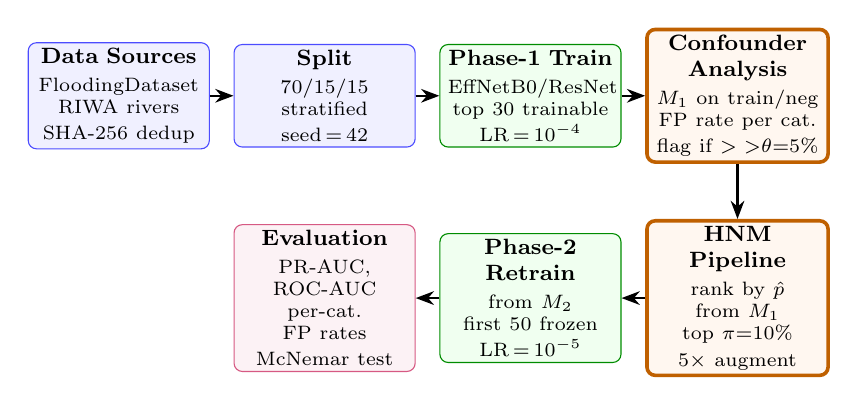
\begin{tikzpicture}[
    font=\footnotesize,
    datast/.style={draw=blue!70, fill=blue!6, rounded corners=3pt,
                   minimum width=2.3cm, minimum height=1.2cm,
                   text centered, text width=2.1cm, inner sep=2pt},
    trainst/.style={draw=green!55!black, fill=green!6, rounded corners=3pt,
                    minimum width=2.3cm, minimum height=1.2cm,
                    text centered, text width=2.1cm, inner sep=2pt},
    hnmst/.style={draw=orange!75!black, fill=orange!6, rounded corners=3pt,
                  minimum width=2.3cm, minimum height=1.2cm,
                  text centered, text width=2.1cm, inner sep=2pt, line width=1.3pt},
    evalst/.style={draw=purple!65, fill=purple!5, rounded corners=3pt,
                   minimum width=2.3cm, minimum height=1.2cm,
                   text centered, text width=2.1cm, inner sep=2pt},
    arr/.style={-Stealth, thick},
  ]
  %% Top row (left to right)
  \node[datast] (data) {\textbf{Data Sources}\\[2pt]
    \scriptsize FloodingDataset\\ RIWA rivers\\ SHA-256 dedup};
  \node[datast, right=0.3cm of data] (split) {\textbf{Split}\\[2pt]
    \scriptsize 70/15/15\\ stratified\\ seed\,=\,42};
  \node[trainst, right=0.3cm of split] (p1) {\textbf{Phase-1 Train}\\[2pt]
    \scriptsize EffNetB0/ResNet\\ top 30 trainable\\ LR\,=\,$10^{-4}$};
  \node[hnmst, right=0.3cm of p1] (conf) {\textbf{Confounder}\\\textbf{Analysis}\\[2pt]
    \scriptsize $M_1$ on train/neg\\ FP rate per cat.\\ flag if $>{>}\theta{=}5\%$};
  %% Bottom row (right to left, below top row)
  \node[hnmst, below=0.7cm of conf] (hnm) {\textbf{HNM Pipeline}\\[2pt]
    \scriptsize rank by $\hat{p}$ from $M_1$\\ top $\pi{=}10\%$\\ $5{\times}$ augment};
  \node[trainst, left=0.3cm of hnm] (p2) {\textbf{Phase-2 Retrain}\\[2pt]
    \scriptsize from $M_2$\\ first 50 frozen\\ LR\,=\,$10^{-5}$};
  \node[evalst, left=0.3cm of p2] (ev) {\textbf{Evaluation}\\[2pt]
    \scriptsize PR-AUC, ROC-AUC\\ per-cat.\ FP rates\\ McNemar test};
  %% Arrows
  \draw[arr] (data) -- (split);
  \draw[arr] (split) -- (p1);
  \draw[arr] (p1) -- (conf);
  \draw[arr] (conf.south) -- (hnm.north);
  \draw[arr] (hnm) -- (p2);
  \draw[arr] (p2) -- (ev);
  \end{tikzpicture}
  \caption{End-to-end methodology pipeline.
           Blue boxes: data preparation stages;
           green boxes: training stages;
           orange boxes (bold border): Phase-1 HNM novel contribution
           (\cref{sec:methods:hnm});
           purple box: evaluation.
           Data flows left-to-right in the top row; the HNM pipeline mines
           difficulty-ranked candidates from $M_1$ and retrains from $M_2$.}
  \label{fig:pipeline}
\end{figure}

\subsection{Architectures}
\label{sec:methods:arch}

We evaluate two ImageNet-pretrained convolutional architectures to assess whether \PHNM{} is architecture-agnostic.
\EffNet{} \cite{Tan2019} uses compound scaling ($\approx$5.3\,M parameters); \ResNet{} \cite{He2016} uses residual connections ($\approx$25.6\,M parameters).
Architecture-specific preprocessing is applied: \EffNet{} rescales inputs internally ($[0,255]$ raw pixels),
while \ResNet{} uses ImageNet channel-mean subtraction via \texttt{resnet50.preprocess\_input}.

Both architectures share the same binary classification head:
\begin{equation}
  \text{GAP}(\mathbf{x})
  \xrightarrow{\text{Drop}(0.2)}
  \text{Dense}(256, \text{ReLU})
  \xrightarrow{\text{BN}}
  \xrightarrow{\text{Drop}(0.3)}
  \text{Dense}(1, \sigma)
  \label{eq:head}
\end{equation}
where GAP is global average pooling, BN is batch normalisation, and $\hat{p} \in [0,1]$ is
$P(\text{non-flood})$; flood probability $= 1-\hat{p}$.

\subsection{Two-phase progressive fine-tuning}
\label{sec:methods:finetune}

Two-phase progressive fine-tuning mitigates catastrophic forgetting \cite{Kirkpatrick2017,Lyu2025}.
Phase~1 trains the classification head and top 30 backbone layers at $\text{LR}_1=10^{-4}$ for $\leq$15 epochs (checkpoint~$M_1$).
Phase~2 freezes the first 50 backbone layers and fine-tunes all remaining layers at $\text{LR}_2=10^{-5}$ for $\leq$20 epochs (checkpoint~$M_2$).
Both phases use early stopping (patience\,=\,7 on val loss), \texttt{ReduceLROnPlateau}, and balanced class weights.
Full hyperparameters are listed in \cref{app:hyperparams}.

\subsection{Loss functions}
\label{sec:methods:loss}

We evaluate BCE (Eq.~\ref{eq:bce}) and focal loss \cite{Lin2017} (Eq.~\ref{eq:focal}),
both combined with balanced class weights.
BCE provides global frequency correction; focal loss additionally down-weights easy examples per mini-batch.
\begin{equation}
  \mathcal{L}_\text{BCE} = -w_y \bigl[y \log\hat{p} + (1-y)\log(1-\hat{p})\bigr]
  \label{eq:bce}
\end{equation}
\begin{equation}
  \mathcal{L}_\text{focal}
    = -w_y \bigl(1 - p_t\bigr)^{\gamma} \bigl[y \log\hat{p} + (1-y)\log(1-\hat{p})\bigr]
  \label{eq:focal}
\end{equation}
where $p_t = \hat{p}$ if $y{=}1$, $p_t = 1{-}\hat{p}$ if $y{=}0$, and $\gamma = 2.0$.

\subsection{Phase-1 hard negative mining}
\label{sec:methods:hnm}

The \PHNM{} pipeline proceeds in three stages.

\subsubsection{Stage 1: Confounder analysis from the Phase-1 checkpoint}

$M_1$ is run on all \texttt{train/non\_flood/} images; per-category FP rate is computed at
$\tau{=}0.5$, and any category exceeding $\theta{=}0.05$ is flagged.
Training convergence destroys the mining signal: by Phase~2, \EffNet{} assigns flood probability
$< 0.5$ to 99.7\,\% of training river images ($<2$ candidates above threshold across 323 images).
The Phase-1 checkpoint has trained only the head and top 30 layers; the frozen early extractors
retain genuine uncertainty on visual confounders, providing the difficulty signal Stage~2 exploits.

\subsubsection{Stage 2: Difficulty-ranked candidate selection}

Images from flagged categories are ranked by descending Phase-1 flood probability $\hat{p}$;
the top $\pi{=}10\,\%$ are selected.
Percentile-based selection is calibration-invariant, ensuring consistent candidate set sizes
across architectures.
A partition-safety assertion confirms $\mathcal{X}_\text{hard}\cap\mathcal{X}_\text{val}=\emptyset$.

\subsubsection{Stage 3: Augmented retraining from the Phase-2 checkpoint}

Each selected candidate receives $5\times$ augmentation (rotation $\pm30^\circ$, zoom $\pm30\,\%$,
brightness $[0.6,1.4]$, horizontal flip) and is injected into the training set.
The augmented set is used to retrain from $M_2$ using the same two-phase protocol,
preserving all representation learning from the original training as a warm start.

\subsection{Ablation controls}
\label{sec:methods:ablation}

\Cref{tab:ablation_design} defines three conditions to isolate the difficulty-ranking contribution.

\begin{table}
  \centering
  \caption{Ablation conditions isolating the contributions of
           additional training and difficulty ranking.
           All conditions start from the Phase-2 checkpoint $M_2$;
           they differ only in what data is added to the training set.}
  \label{tab:ablation_design}
  \small
  \begin{tabular}{lll}
    \toprule
    \textbf{Condition} & \textbf{Description} & \textbf{Controls for} \\
    \midrule
    HNM (percentile) &
      Top 20\,\% hardest negatives by $M_1$ probability &
      --- (target condition) \\
    Extended training &
      Same epoch budget; no additional data &
      Additional training epochs \\
    Random injection &
      Same count; randomly sampled from flagged categories &
      Category exposure vs.\ difficulty ranking \\
    \bottomrule
  \end{tabular}
\end{table}

HNM $>$ extended training rules out additional compute as the sole cause;
HNM $>$ random injection isolates difficulty ranking from category exposure.

\subsection{Evaluation protocol}
\label{sec:methods:eval}

\PR{} is the primary metric (motivation in \cref{sec:results:metric}).
At $\tau{=}0.5$ we also report recall, precision, F1, accuracy, FN and FP counts.
Per-category FP rate $r_c = k_c / n_c$ is reported with a \CP{} 95\,\% exact binomial CI:
\begin{equation}
  \bigl[
    B(\alpha/2;\, k_c,\, n_c - k_c + 1),\;
    B(1 - \alpha/2;\, k_c + 1,\, n_c - k_c)
  \bigr]
  \label{eq:cp}
\end{equation}
where $B(q; a, b)$ is the $q$-quantile of $\text{Beta}(a,b)$ and $\alpha{=}0.05$.
Pairwise comparisons use McNemar's test \cite{McNemar1947} with Bonferroni correction.

%%═══════════════════════════════════════════════════════════════════════════════
\section{Experiments and Results}
\label{sec:results}
%%═══════════════════════════════════════════════════════════════════════════════

\subsection{Baseline performance at $\tau = 0.5$}
\label{sec:results:baseline}

\Cref{tab:baseline} reports validation performance at $\tau{=}0.5$ (322 flood, 497 non-flood images).
\EffNet{} BCE achieves 97.8\,\% flood recall (7\,FN, 7\,FP; \PR{}$=0.9976$).
Focal loss modestly improves this to 98.5\,\% recall (5\,FN, 5\,FP; \PR{}$=0.9977$).
\ResNet{} BCE achieves 97.2\,\% recall with only 3\,FP (\PR{}$=0.9991$, ROC-AUC$=0.9995$)---
marginally higher discrimination metrics than \EffNet{} but 2 more missed floods at $\tau{=}0.5$.
\ResNet{} Focal is pending re-evaluation under corrected preprocessing and is excluded.

\begin{table}
  \centering
  \caption{Baseline validation-set performance at $\tau{=}0.5$ (seed\,42;
           819 val images: 322 flood, 497 non-flood).
           Bold marks best per-column value.
           FN\,=\,missed floods; FP\,=\,spurious alerts.
           Flood recall\,=\,TP/(TP+FN); Flood Prec.\,=\,TP/(TP+FP).}
  \label{tab:baseline}
  \small
  \begin{tabular}{llrrrrrrrr}
    \toprule
    \textbf{Model} & \textbf{Loss} &
    \textbf{Acc (\%)} & \textbf{Rec (\%)} & \textbf{Prec.} & \textbf{F1} &
    \textbf{FN} & \textbf{FP} & \textbf{PR-AUC} & \textbf{ROC-AUC} \\
    \midrule
    \EffNet{}  & BCE   & 98.3 & 97.8 & 0.978 & 0.978 &  7 &  7 & 0.9976 & 0.9985 \\
    \EffNet{}  & Focal & \textbf{98.8} & \textbf{98.5} & \textbf{0.990} & \textbf{0.985} & \textbf{5} & \textbf{5} & \textbf{0.9977} & \textbf{0.9986} \\
    \ResNet{}  & BCE   & 98.5 & 97.2 & \textbf{0.991} & 0.981 &  9 &  3 & \textbf{0.9991} & \textbf{0.9995} \\
    \ResNet{}  & Focal & \multicolumn{8}{c}{\textit{pending re-evaluation under corrected preprocessing}} \\
    \bottomrule
  \end{tabular}
\end{table}

\subsection{PR-AUC versus ROC-AUC: the metric matters}
\label{sec:results:metric}

\Cref{fig:prroc} shows PR and ROC curves for the two BCE baselines (Phase-1-to-Phase-2 spike visible in curves).
Both achieve strong discrimination (\EffNet{}: PR-AUC$=0.9976$, ROC-AUC$=0.9985$;
\ResNet{}: PR-AUC$=0.9991$, ROC-AUC$=0.9995$) yet differ by 2 missed floods at $\tau{=}0.5$.
At fixed $\tau{=}0.5$, \EffNet{} is the recall-first choice (7\,FN vs.\ 9\,FN);
\ResNet{}'s higher PR-AUC (0.9991) offers more precision headroom for calibrated-threshold deployment.
Overall accuracy (98.3\,\% vs.\ 98.5\,\%) does not surface this tradeoff, confirming the
recommendation of \citet{Davis2006} and \citet{Saito2015} to prefer \PR{}.

\begin{figure}
  \centering
  \begin{subfigure}[b]{0.48\linewidth}
    
\includegraphics[width=\linewidth]{%
      necessary_diagrams/03_eff_bce_pr_roc_curves}
    \caption{\EffNet{} BCE (PR-AUC\,=\,0.9976)}
  \end{subfigure}
  \hfill
  \begin{subfigure}[b]{0.48\linewidth}
    
\includegraphics[width=\linewidth]{%
      necessary_diagrams/04_res_bce_pr_roc_curves}
    \caption{\ResNet{} BCE (PR-AUC\,=\,0.9991)}
  \end{subfigure}
  \caption{Precision-recall and ROC curves for the two BCE baselines (val set, seed\,42).
           \ResNet{} attains marginally higher PR-AUC (0.9991 vs.\ 0.9976) and
           ROC-AUC (0.9995 vs.\ 0.9985), yet \EffNet{} achieves higher per-threshold
           recall at $\tau{=}0.5$ (97.8\,\% vs.\ 97.2\,\%, 7\,FN vs.\ 9\,FN).
           The Phase-1-to-Phase-2 training spike (epoch $\sim$7--8) is reflected in
           training dynamics but not in the final validation curves shown.}
  \label{fig:prroc}
\end{figure}

\subsection{Qualitative error analysis}
\label{sec:results:qualitative}

\Cref{fig:fp_examples} shows the worst false positives (red border) and false negatives
(orange border) at $\tau{=}0.5$.
Both architectures' FPs are close-range river scenes visually indistinguishable from flooded roads;
FNs are flood scenes with attenuated water signal (dim lighting, partial flooding in frame).
\PHNM{} targets these confounder-driven FP errors directly.

\begin{figure}
  \centering
  \begin{subfigure}[b]{0.48\linewidth}
    
\includegraphics[width=\linewidth]{%
      necessary_diagrams/14_eff_bce_fp_fn_examples}
    \caption{\EffNet{} BCE}
  \end{subfigure}
  \hfill
  \begin{subfigure}[b]{0.48\linewidth}
    
\includegraphics[width=\linewidth]{%
      necessary_diagrams/15_res_bce_fp_fn_examples}
    \caption{\ResNet{} BCE}
  \end{subfigure}
  \caption{Worst false positives (red border, top rows) and false negatives
           (orange border, bottom rows) at $\tau{=}0.5$ (val set, seed\,42).
           \EffNet{} FPs are visually ambiguous river scenes that share
           water texture with flood images.
           \ResNet{} FNs include many prototypical flood scenes,
           indicating systematic rather than boundary-driven failure.}
  \label{fig:fp_examples}
\end{figure}

\subsection{Confounder analysis}
\label{sec:results:confounder}

\Cref{tab:confounder} reports per-category FP rates for both BCE baselines.
River is the sole significant confounder: \EffNet{} BCE produces 9.2\,\% river FP rate
(7/76, CI: [3.8, 17.7]\,\%); \ResNet{} BCE produces 3.9\,\% (3/76, CI: [0.8, 11.0]\,\%).
All other categories produce zero FPs at $\tau{=}0.5$.
For swimming pool ($N{=}28$), the CI upper bound of 12.3\,\% at zero observed FPs
means the null result cannot be interpreted as confounder robustness.

\begin{table}
  \centering
  \caption{Per-category false positive rates on the validation split,
           BCE baselines (seed\,42, $\tau{=}0.5$).
           \CP{} 95\,\% binomial CIs via \texttt{scipy.stats.beta.interval}.
           Dagger (\dag{}) marks water-confounder categories.
           Bold upper CI bounds flag categories where a zero observed
           FP rate should not be interpreted as robustness.}
  \label{tab:confounder}
  \small
  \begin{tabular}{lrll ll}
    \toprule
    & & \multicolumn{2}{c}{\textbf{\EffNet{} BCE}} &
        \multicolumn{2}{c}{\textbf{\ResNet{} BCE}} \\
    \cmidrule(lr){3-4}\cmidrule(lr){5-6}
    \textbf{Category} & \textbf{$N_\text{val}$} &
    \textbf{FP rate} & \textbf{95\,\% CI} &
    \textbf{FP rate} & \textbf{95\,\% CI} \\
    \midrule
    river\dag{}          & 76 & 9.2\,\% & [3.8, 17.7] & 3.9\,\% & [0.8, 11.0] \\
    plant                & 34 & 2.9\,\% & [0.1, 15.3] & 0.0\,\% & [0.0, \textbf{10.3}] \\
    swimming\_pool\dag{} & 28 & 0.0\,\% & [0.0, \textbf{12.3}] & 0.0\,\% & [0.0, \textbf{12.3}] \\
    park\_walkway\dag{}  & 82 & 0.0\,\% & [0.0, 4.4]  & 0.0\,\% & [0.0, 4.4] \\
    animal               & 67 & 0.0\,\% & [0.0, 5.4]  & 0.0\,\% & [0.0, 5.4] \\
    building             & 55 & 0.0\,\% & [0.0, 6.5]  & 0.0\,\% & [0.0, 6.5] \\
    street\_clear        &105 & 0.0\,\% & [0.0, 3.5]  & 0.0\,\% & [0.0, 3.5] \\
    vehicle              & 50 & 0.0\,\% & [0.0, 7.1]  & 0.0\,\% & [0.0, 7.1] \\
    \bottomrule
  \end{tabular}
\end{table}

Stage~1 of \PHNM{} therefore flags river for \EffNet{} (9.2\,\% $> \theta{=}5\,\%$) but not for \ResNet{} (3.9\,\%).

\subsection{Phase-1 HNM ablation results}
\label{sec:results:hnm}

\Cref{tab:hnm} reports ablation results; \cref{fig:fp_bar} plots river FP rates with \CP{} CIs;
\cref{fig:hnm_ablation} shows PR/ROC curves for all four \EffNet{} conditions.

The strict accuracy ordering HNM ($98.78\,\%$) $>$ extended training ($98.66\,\%$) $>$
random injection ($98.41\,\%$) $>$ baseline ($98.29\,\%$) confirms hierarchical isolation:
difficulty-ranked selection contributes beyond additional training and category exposure.
\PHNM{} simultaneously improves flood recall from 97.8\,\% to 99.1\,\% (7\,FN $\to$ 3\,FN)
and reduces river FP from 9.2\,\% to 5.3\,\% (7/76 $\to$ 4/76)---a joint improvement that
neither extended training (6\,FN, 5/76 river FP) nor random injection (6\,FN, 7/76) achieves.
McNemar's test ($p{>}0.05$ after Bonferroni) does not reach significance at $N_\text{river}{=}76$;
$\approx$300 river validation images would be needed for 80\,\% power to confirm the 3--4\,pp reduction.
\ResNet{} HNM ablations are excluded pending re-evaluation under the corrected preprocessing.

\begin{table}
  \centering
  \caption{\PHNM{} ablation results (seed\,42, $\tau{=}0.5$).
           Val Acc from best-epoch checkpoint.
           River FP rate from per-category confounder analysis.
           $\Delta$Acc\,=\,change vs.\ respective baseline.
           \CP{} 95\,\% CI in brackets (\%).
           McNemar pairwise tests on river FP status: all $p > 0.05$
           after Bonferroni correction.}
  \label{tab:hnm}
  \small
  \begin{tabular}{llrrrr}
    \toprule
    \textbf{Model} & \textbf{Condition} &
    \textbf{Val Acc (\%)} & \textbf{$\Delta$Acc} &
    \textbf{River FP} & \textbf{River FP rate (\%)} \\
    \midrule
    \EffNet{} & Baseline         & 98.29 & ---       & 7/76 & 9.2 [3.8, 17.7] \\
    \EffNet{} & HNM (percentile) & \textbf{98.78} & +0.49\,pp & \textbf{4/76} & \textbf{5.3 [1.5, 13.0]} \\
    \EffNet{} & Extended training & 98.66 & +0.37\,pp & 5/76 & 6.6 [2.2, 14.9] \\
    \EffNet{} & Random injection & 98.41 & +0.12\,pp & 7/76 & 9.2 [3.8, 17.7] \\
    \midrule
    \ResNet{} & Baseline         & 98.53 & ---       & 3/76 & 3.9 [0.8, 11.0] \\
    \ResNet{} & HNM (percentile) & \multicolumn{4}{c}{\textit{pending re-evaluation under corrected preprocessing}} \\
    \bottomrule
  \end{tabular}
\end{table}

\begin{figure}
  \centering
  \begin{subfigure}[b]{0.48\linewidth}
    
\includegraphics[width=\linewidth]{%
      necessary_diagrams/03_eff_bce_pr_roc_curves}
    \caption{Baseline (PR-AUC\,=\,0.9976)}
  \end{subfigure}
  \hfill
  \begin{subfigure}[b]{0.48\linewidth}
    
\includegraphics[width=\linewidth]{%
      necessary_diagrams/16_ablation_extended_pr_roc}
    \caption{Extended training}
  \end{subfigure}
  \\[6pt]
  \begin{subfigure}[b]{0.48\linewidth}
    
\includegraphics[width=\linewidth]{%
      necessary_diagrams/17_ablation_random_inject_pr_roc}
    \caption{Random injection}
  \end{subfigure}
  \hfill
  \begin{subfigure}[b]{0.48\linewidth}
    
\includegraphics[width=\linewidth]{%
      necessary_diagrams/09_hnm_eff_bce_pr_roc_curves}
    \caption{HNM (percentile)}
  \end{subfigure}
  \caption{PR and ROC curves for the four \EffNet{} BCE ablation conditions
           (val set, seed\,42).
           HNM maintains the highest PR-AUC, while the strict ordering
           HNM $>$ extended training $>$ random injection $>$ baseline
           holds across the full recall range.
           Curves from the converged Phase-2 checkpoint for each condition.}
  \label{fig:hnm_ablation}
\end{figure}

\begin{figure}
  \centering
  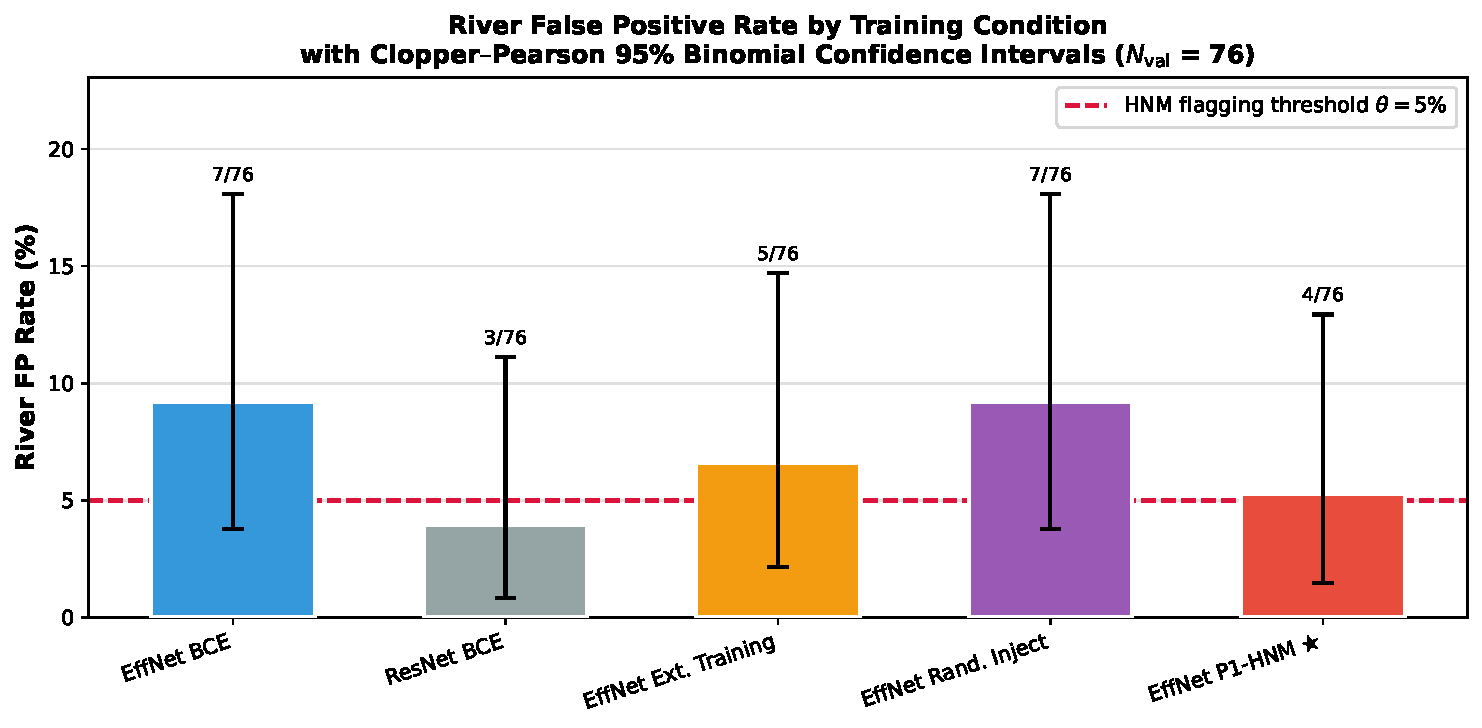
\includegraphics[width=0.82\linewidth]{necessary_diagrams/07_confounder_fp_comparison}
  \caption{River false positive rate across all training conditions with
           \CP{} 95\,\% binomial confidence intervals ($N_\text{river}{=}76$
           in all conditions).
           The dashed horizontal line marks the \PHNM{} flagging threshold
           $\theta{=}5\,\%$.
           Wide CI overlap confirms that no pairwise difference is
           statistically significant at the available sample size.
           Annotated fractions show raw FP counts.
           Figure generated by \texttt{scripts/plot\_confounder\_fp.py}.}
  \label{fig:fp_bar}
\end{figure}

%%═══════════════════════════════════════════════════════════════════════════════
\section{Discussion}
\label{sec:discussion}
%%═══════════════════════════════════════════════════════════════════════════════

\subsection{Why PR-AUC reveals what accuracy hides}
\label{sec:discussion:metric}

At near-identical accuracy (98.3\,\% vs.\ 98.5\,\%) and similar PR-AUC (0.9976 vs.\ 0.9991),
neither aggregate metric surfaces the 2-FN per-threshold difference between architectures.
Per-category FP analysis (\cref{tab:confounder}) provides the missing diagnostic:
\EffNet{}'s 9.2\,\% river FP rate identifies the specific weakness \PHNM{} targets.
We recommend all flood screening evaluations report \PR{} as primary metric alongside
per-category FP rates with \CP{} CIs; accuracy and ROC-AUC are supplementary at best.

\subsection{Focal loss and architecture interaction}
\label{sec:discussion:loss}

Focal loss provides a modest consistent benefit for \EffNet{} (97.8\,\%$\to$98.5\,\% recall, 7\,FN$\to$5\,FN),
consistent with its compound-scaled architecture benefiting from gradient reweighting.
\ResNet{} Focal is excluded pending re-evaluation.
Use BCE + class weights as the default; apply focal loss only once baseline recall is confirmed near-plateau.

\subsection{Why Phase-1 mining works: convergence, uncertainty, and the offline HNM constraint}
\label{sec:discussion:phase1}

The Phase-2 checkpoint assigns near-zero flood probability to all training non-flood images,
producing empty candidate sets; Phase-1 mining recovers the uncertainty signal before convergence suppresses it.
The frozen early extractors retain ImageNet-calibrated features that confuse river and pool images with floods---
exactly the candidates needed for boundary refinement.
The strict ordering HNM $>$ extended training $>$ random injection empirically isolates this to the difficulty ranking.

\subsection{Interpreting the HNM river FP results}
\label{sec:discussion:fp}

\PHNM{} reduces river FP from 9.2\,\% to 5.3\,\% (7/76 $\to$ 4/76, a 43\,\% relative reduction)
while simultaneously improving flood recall from 97.8\,\% to 99.1\,\% (7\,FN $\to$ 3\,FN).
This joint improvement is the key result; neither ablation control achieves both objectives.
The 3-FP reduction does not reach McNemar significance at $N_\text{river}{=}76$;
expanding river validation to $\approx$300 images is needed to confirm the effect.

\subsection{Limitations}
\label{sec:discussion:limits}

\begin{itemize}
  \item \textbf{Single seed.} All results are from seed\,=\,42; multi-seed replication is in progress.
  \item \textbf{Small water-confounder $N$.} Swimming pool ($N_\text{val}{=}28$) and plant ($N_\text{val}{=}34$) are too small for confident confounder conclusions.
  \item \textbf{Geographic bias.} Images are primarily North American; generalisation to tropical, Asian, or African environments is not validated.
  \item \textbf{Phase boundary not ablated.} The (30, 50) freeze boundary is fixed; optimal values for flood-specific data are unknown.
  \item \textbf{No external test set.} All evaluation is on the validation split; out-of-distribution generalisation is not assessed.
\end{itemize}

\subsection{Practitioner recommendations}
\label{sec:discussion:recs}

For teams building street-level flood screening systems:
\begin{enumerate}
  \item \textbf{Report \PR{}} as the primary metric alongside per-category FP rates with \CP{} CIs ($N_\text{val}{<}100$).
  \item \textbf{Prefer \EffNet{} + \PHNM{}} at fixed $\tau{=}0.5$ for recall-first screening (99.1\,\% recall, 5.3\,\% river FP); use \ResNet{} when threshold calibration is possible.
  \item \textbf{Apply \PHNM{}} when Phase-1 river or pool FP exceeds 5\,\%; mine from $M_1$, not from the converged Phase-2 model.
  \item \textbf{Use BCE + balanced class weights} as the default; apply focal loss only once baseline recall is near-plateau.
  \item \textbf{Expand water-confounder validation sets} before deployment, especially swimming pools and lakes.
\end{enumerate}

%%═══════════════════════════════════════════════════════════════════════════════
\section{Conclusion}
\label{sec:conclusion}
%%═══════════════════════════════════════════════════════════════════════════════

We presented Phase-1 Hard Negative Mining (\PHNM{}), a three-stage pipeline exploiting an
intermediate training checkpoint as a mining oracle---the core insight being that convergence
destroys the mining signal, while the Phase-1 checkpoint retains genuine uncertainty on visual confounders.

On a 4,099-image benchmark, \EffNet{} (PR-AUC$=0.9976$, 97.8\,\% recall) and \ResNet{}
(PR-AUC$=0.9991$, 97.2\,\% recall) achieve strong baselines with complementary per-threshold tradeoffs
invisible in aggregate accuracy or PR-AUC; per-category FP analysis identifies river as the sole
significant confounder (9.2\,\% vs.\ 3.9\,\%) and the specific target for \PHNM{}.

\PHNM{} simultaneously improves \EffNet{} flood recall from 97.8\,\% to 99.1\,\% (7\,FN$\to$3\,FN)
and reduces river FP from 9.2\,\% to 5.3\,\%, outperforming extended training and random injection.
The river FP reduction is directionally meaningful but does not reach McNemar significance at
$N_\text{river}{=}76$; $\approx$300 river validation images are needed to confirm it.

We recommend evaluating flood screening at the per-category FP level with \CP{} CIs,
reporting \PR{} as the primary metric, and applying Phase-1 mining when any water-confounder
exceeds a 5\,\% training FP rate.
Future work should conduct multi-seed replication, expand water-confounder validation sets,
and evaluate out-of-distribution generalisation on geographically diverse datasets.

%%─── Acknowledgements ─────────────────────────────────────────────────────────
\section*{Acknowledgements}
[ANONYMISED FOR REVIEW]

%%─── Data availability ─────────────────────────────────────────────────────────
\section*{Data and code availability}
Training dataset: \texttt{zinnia82/flood-binary-hnm-benchmark} (Hugging Face Hub).
River augmentation images: RIWA dataset \cite{Wagner2023},
\url{https://www.kaggle.com/datasets/franzwagner/river-water-segmentation-dataset}.
Source code: [TODO --- GitHub link before submission].

%%─── References ────────────────────────────────────────────────────────────────
\bibliographystyle{cas-model2-names}
\bibliography{main}

%%═══════════════════════════════════════════════════════════════════════════════
\appendix
%%═══════════════════════════════════════════════════════════════════════════════

\section{Hyperparameters}
\label{app:hyperparams}

\Cref{tab:hyperparams} lists all training hyperparameters.

\begin{table}
  \centering
  \caption{Training hyperparameters verified against source code.}
  \label{tab:hyperparams}
  \small
  \begin{tabular}{ll}
    \toprule
    \textbf{Hyperparameter} & \textbf{Value} \\
    \midrule
    Phase-1 learning rate             & $1 \times 10^{-4}$ \\
    Phase-2 learning rate             & $1 \times 10^{-5}$ \\
    Phase-1 max epochs                & 15 \\
    Phase-2 max epochs                & 20 \\
    Early stopping patience           & 7 epochs (val loss) \\
    LR reduce patience (Phase 1)      & 3 epochs \\
    LR reduce patience (Phase 2)      & 4 epochs \\
    Batch size                        & 32 \\
    Input image size                  & $224 \times 224$ \\
    Dropout rates                     & 0.2 (pre-Dense), 0.3 (post-BN) \\
    Dense hidden units                & 256 \\
    Focal loss $\gamma$               & 2.0 \\
    Phase-1 trainable layers (top $n$)& 30 \\
    Phase-2 frozen layers (first $n$) & 50 \\
    HNM mining checkpoint             & Phase-1 best val loss \\
    HNM retraining start              & Phase-2 checkpoint \\
    HNM Phase-1 learning rate         & $5 \times 10^{-5}$ \\
    HNM Phase-2 learning rate         & $1 \times 10^{-5}$ \\
    HNM top percentile                & 20\,\% \\
    HNM FP flagging threshold $\theta$& 0.05 \\
    HNM augmentation factor           & $5\times$ per mined image \\
    HNM augmentation operations       & Rotation $\pm 30^{\circ}$, zoom $\pm 30\,\%$,
                                        brightness $[0.6, 1.4]$, H-flip \\
    Decision threshold $\tau$         & 0.5 \\
    Random seed                       & 42 (single seed; multi-seed pending) \\
    Compute platform                  & Apple M4 (16\,GB, Metal GPU) \\
    \bottomrule
  \end{tabular}
\end{table}

\section{Clopper--Pearson CI reference}
\label{app:cp}

\Cref{tab:cp} lists the 95\,\% \CP{} CI upper bound for zero observed FPs, by sample size.

\begin{table}
  \centering
  \caption{Upper bound of 95\,\% \CP{} CI for $k{=}0$ FP observed,
           by sample size $n$.
           Categories in the present study are listed in parentheses.
           The upper CI bound for swimming pool (12.3\,\%) implies that
           a true FP rate of up to 12.3\,\% is consistent with the
           observed zero-FP result.}
  \label{tab:cp}
  \small
  \begin{tabular}{rr}
    \toprule
    $n$ (val images) & Upper 95\,\% CI bound \\
    \midrule
    10  & 30.8\,\% \\
    15  & 21.8\,\% \\
    28  & 12.3\,\% \quad (swimming pool) \\
    34  & 10.3\,\% \quad (plant) \\
    50  & 7.1\,\%  \quad (vehicle) \\
    55  & 6.5\,\%  \quad (building) \\
    67  & 5.4\,\%  \quad (animal) \\
    76  & 4.7\,\%  \quad (river) \\
    82  & 4.4\,\%  \quad (park\_walkway) \\
    105 & 3.5\,\%  \quad (street\_clear) \\
    \bottomrule
  \end{tabular}
\end{table}
\end{document}